
\documentclass{standalone}

%\documentclass[convert]{standalone}
% convert: in addition to pdf output files, png files are created
% convert options does work properly with -output-directory option of latexmk

\usepackage{tikz-feynman}
\tikzfeynmanset{compat=1.1.0}


\begin{document}
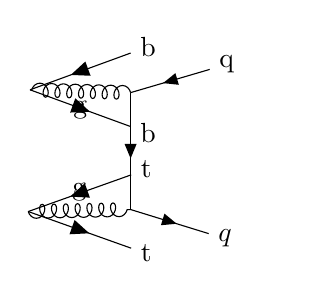
\begin{tikzpicture}
          \begin{feynman}
            \diagram [small, vertical=a to b] {
            % t-channel ttbar, qq -> gg -- > bbtt

            qi1 [particle=q] -- [fermion] a -- [gluon, edge label=g] g1,
            %qi2 [particle=q]  -- b -- [gluon, edge label=g] g2,
            g2 -- [gluon, edge label=g] b -- [fermion] qi2 [particle=\( q \)] ,

            a -- [fermion] b,

            % invisible helper
            qi1 -- [draw=none] invis -- [draw=none] qi2,
            g1 -- [draw=none] g2,
            };

            \vertex [right=of g1] (b12_invis_helper);    % helper
            \vertex [above=0.3cm of b12_invis_helper] (b1) {b};
            \vertex [below=0.3cm of b12_invis_helper] (b2) {b};
            \draw [fermion] (b1) -- (g1);
            \draw [fermion] (g1) -- (b2);

            \vertex [right=of g2] (t12_invis_helper);    % helper
            \vertex [above=0.3cm of t12_invis_helper] (t1) {t};
            \vertex [below=0.3cm of t12_invis_helper] (t2) {t};
            \draw [fermion] (t1) -- (g2);
            \draw [fermion] (g2) -- (t2);
          \end{feynman}
        \end{tikzpicture}
\end{document}
